\documentclass[11pt]{article}
\usepackage[margin=1in]{geometry}
\usepackage{amsmath,amssymb,amsthm}
\usepackage{algorithm,algpseudocode}
\usepackage{graphicx}
\usepackage{hyperref}
\usepackage{booktabs}
\usepackage{enumitem}
\usepackage{tikz}
\usetikzlibrary{arrows.meta,positioning,calc}

\newtheorem{theorem}{Theorem}
\newtheorem{lemma}[theorem]{Lemma}
\newtheorem{corollary}[theorem]{Corollary}
\newtheorem{proposition}[theorem]{Proposition}
\newtheorem{definition}{Definition}
\newtheorem{remark}{Remark}
\newtheorem{example}{Example}

\title{Practical Livelock Analysis\\in Parameterized Unidirectional Rings}
\author{Aly Farahat}
\date{}

\begin{document}
\maketitle

\begin{abstract}
We develop a practical framework for livelock analysis in parameterized unidirectional rings. Klinkhamer and Ebnenasir established that livelock detection is $\Sigma^0_1$-complete via reduction from the NW-deterministic periodic domino problem~\cite{mazoyer-rapaport}. We observe that lifting the analysis to the space of transition--witness pairs reveals structure that supports effective verification.

We construct a \emph{product transition graph} $G_\times(T)$ (at most $|T|^2$ nodes) whose cycles capture the pairwise equivariant structure underlying all livelocks. The maximal witness-closed subgraph $G^*(T)$ is computable in polynomial time. When $G^*(T) = \emptyset$, the protocol is provably livelock-free for all ring sizes. When $G^*(T) \neq \emptyset$, a backtracking search over simple cycles detects livelocks whose closing chains consist of simple cycles.

We demonstrate via an explicit counterexample---a forced binary counter converted through the K\&E gadget---that livelocks can exist through compound-only closing chains where no simple cycle backward-closes. This is consistent with the $\Sigma^0_1$-completeness of livelock detection. Despite this theoretical limitation, the semi-algorithm terminates on every input with one of three outcomes (\textsc{Free}, \textsc{Livelock}, \textsc{Inconclusive}). Across 4{,}349 protocols tested---including random self-disabling protocols and Wang tile gadgets---the \textsc{Free} and \textsc{Livelock} outcomes have zero errors. The \textsc{Inconclusive} outcome occurs correctly on Kari's aperiodic tiles (livelock-free) and on the forced counter (livelock via compound chains). No protocol designed for self-stabilization has ever produced an \textsc{Inconclusive} result.

We extend to non-self-disabling protocols via burst closure. Python implementation at \url{https://github.com/cosmoparadox/mathematical-tools}.
\end{abstract}

%% ============================================================
\section{Introduction}
\label{sec:intro}
%% ============================================================

Self-stabilization~\cite{dijkstra1974} guarantees that a distributed system recovers from arbitrary transient faults to a legitimate configuration, regardless of the initial state. A key obstacle to self-stabilization in ring protocols is \emph{livelock}: an infinite execution in which processes continually change state but never reach legitimacy. Determining whether a given protocol admits a livelock---for any ring size---is a fundamental parameterized verification problem.

\paragraph{Background.} Klinkhamer and Ebnenasir~\cite{klinkhamer-ebnenasir} established that livelock detection for parameterized rings of self-disabling processes is $\Sigma^0_1$-complete and livelock-freedom verification is $\Pi^0_1$-complete, via a reduction from the NW-deterministic periodic domino problem~\cite{mazoyer-rapaport}. Their torus characterization---the equivalence between livelocks and doubly-periodic tilings---is foundational and underlies our work. Notably, they also showed that the \emph{synthesis} of self-stabilizing rings is decidable~\cite{klinkhamer-ebnenasir}, and Farahat's equivariance framework~\cite{farahat-diss} has been used to prove livelock freedom of difficult protocols such as Dijkstra's self-stabilizing token ring~\cite{gouda-haddix}.

\paragraph{Parameterized verification context.} Approaches to parameterized verification of undecidable problems fall broadly into two categories~\cite{bloem-survey}: (i)~identifying decidable subclasses through cutoff bounds~\cite{emerson-namjoshi} or well-structured transition systems, which guarantee termination but restrict the class of systems; and (ii)~developing semi-decision procedures such as regular model checking or bounded model checking, which handle broader classes but provide no termination guarantee. In practice, the line between these approaches blurs: semi-decision procedures often serve as decision procedures on the fragments that arise in practice. Our work occupies this middle ground. Unlike typical semi-decision procedures that verify only one direction (finding a bug or proving correctness), our framework provides polynomial-time certificates in \emph{both} directions: $G^* = \emptyset$ certifies livelock-freedom, and closing cycles certify livelock existence. Only the genuinely undecidable boundary---aperiodic structures and compound-only closing chains---produces the \textsc{Inconclusive} outcome.

\paragraph{Our observation.} Building on Klinkhamer and Ebnenasir's torus characterization, we observe that lifting the analysis from individual transitions to \emph{pairs} of transitions reveals structure that supports effective verification. A single transition cycle does not determine when equivariant closure occurs: equivariance fixes the predecessor's own and wr values (its H-walk), but not its pred values, which select specific transitions from $T$. Different pred assignments yield different witness cycles, which close at different periods---or not at all.

We construct a \emph{product graph} over transition--witness pairs---at most $|T|^2$ nodes---that captures the equivariant structure. A pair commits to specific transitions at every position, including pred values, so its equivariant period is determined. Every livelock maps into the product graph (Theorem~\ref{thm:necessary}), producing a witness-closed subgraph. The product graph's simple cycles---of length at most $|T|^2$---identify equivariant pairs that are candidates for generating livelocks via backward propagation.

The maximal witness-closed subgraph $G^*(T)$ is computable in polynomial time. When $G^* = \emptyset$, the protocol is provably livelock-free for all ring sizes. When $G^* \neq \emptyset$, backward propagation of simple cycles through $G^*$ serves as a sound livelock detector: any cycle whose backward chain closes in $G^*$ generates a genuine livelock.

\paragraph{Our contribution.}
\begin{enumerate}[nosep]
\item \emph{Necessary condition.} Every livelock maps into the product graph as a witness-closed subgraph (Theorem~\ref{thm:necessary}). Consequently, $G^*(T) = \emptyset$ implies livelock-freedom for all ring sizes, providing a polynomial-time livelock-freedom verifier.

\item \emph{Sufficient condition.} Any simple cycle in $G^*$ whose backward chain closes generates a genuine livelock (Theorem~\ref{thm:sufficient}).

\item \emph{Counterexample.} We construct an explicit NW-deterministic Wang tile set (a forced binary counter) whose livelock exists only through compound closing chains---no simple cycle backward-closes (Section~\ref{sec:discussion}). This demonstrates that compound walks can exhibit topology-breaking backward maps, and that the semi-algorithm is necessarily incomplete, consistent with the $\Sigma^0_1$-completeness of livelock detection~\cite{mazoyer-rapaport}.

\item \emph{Semi-algorithm and empirical validation.} A two-phase semi-algorithm---polynomial-time $G^*$ computation followed by backtracking---always terminates with one of three outcomes: \textsc{Free} (livelock-free, certified), \textsc{Livelock} (livelock exists, certified), or \textsc{Inconclusive} (cannot determine). Unlike PROP~\cite{klinkhamer-tr}, which is a pure semi-decider that may run indefinitely, our semi-algorithm always terminates. Across 4{,}349 protocols tested, the \textsc{Free} and \textsc{Livelock} outcomes have zero errors. No protocol designed for self-stabilization has ever produced the \textsc{Inconclusive} outcome.

\item \emph{Extensions.} We extend to non-self-disabling protocols via burst closure (Section~\ref{sec:non-sd}) and to $(1,1)$-asymmetric protocols (Section~\ref{sec:asymmetry}).
\end{enumerate}

\paragraph{Scope.} This paper does not decide livelock detection in general---Mazoyer and Rapaport~\cite{mazoyer-rapaport} established that the NW-deterministic periodic domino problem is undecidable, and Klinkhamer and Ebnenasir~\cite{klinkhamer-ebnenasir} showed this implies $\Sigma^0_1$-completeness of livelock detection. Instead, the product graph provides: (1)~a polynomial-time \emph{complete certificate} for livelock-freedom ($G^* = \emptyset$), (2)~a sound detector for livelocks whose closing chains consist of simple cycles, and (3)~a terminating semi-algorithm that, unlike the pure semi-decider PROP, always returns a definite answer---including \textsc{Inconclusive} when it cannot determine the outcome. This distinguishes our approach: it captures both positive cases (livelock detected) and negative cases (livelock-freedom certified), with \textsc{Inconclusive} reserved for the genuinely hard cases.

%% ============================================================
\section{Definitions}
\label{sec:defs}
%% ============================================================

\subsection{Unidirectional Ring Protocols}

A \emph{unidirectional ring} of size $K$ consists of processes $P_0, P_1, \ldots, P_{K-1}$ arranged in a directed cycle. Each process $P_i$ maintains a state variable $v_i \in \mathbb{Z}_m = \{0, 1, \ldots, m-1\}$ and can read $v_i$ and $v_{i-1 \bmod K}$.

\begin{definition}[Transition]
A \emph{transition} is a triple $t = (p, o, w) \in \mathbb{Z}_m^3$, meaning: if the predecessor's value is $p$ and the process's own value is $o$, the process may write $w$. We call $p$ the \emph{pred value}, $o$ the \emph{own value}, and $w$ the \emph{written value}.
\end{definition}

\begin{definition}[Self-disabling]
A protocol $T$ is \emph{self-disabling} if for every transition $(p, o, w) \in T$, there is no transition $(p, w, u) \in T$ for any $u$. That is, after a process fires $(p, o, w)$, it cannot fire again while the predecessor's value remains $p$---it must wait for an intervening state change from the predecessor. Throughout this paper, all protocols are self-disabling.
\end{definition}

\begin{definition}[Protocol]
A \emph{protocol} is a finite self-disabling set $T \subseteq \mathbb{Z}_m^3$. A transition $(p, o, w) \in T$ is \emph{enabled} at process $P_i$ in configuration $(v_0, \ldots, v_{K-1})$ if $v_{i-1} = p$ and $v_i = o$.
\end{definition}

\begin{definition}[Livelock]
A \emph{livelock} is a global periodic execution of a ring: $K$ processes fire transitions indefinitely, returning the entire ring to the same global configuration after $N$ steps, without ever reaching a legitimate state. As shown by Klinkhamer and Ebnenasir~\cite{klinkhamer-ebnenasir}, a livelock is equivalently a valid tiling of a $K \times N$ torus, where each row is a closed walk of local transitions executed by one process, and adjacent rows satisfy the equivariance conditions (Section~\ref{sec:product}). The walk length $N$ is the \emph{local period}; the number of processes $K$ is the \emph{ring size}.
\end{definition}

\subsection{The $(l,q)$-Asymmetry Model}

\begin{definition}[$(l,q)$-asymmetry]
A ring protocol has $(l,q)$-asymmetry if there are $l$ \emph{distinguished} process types (each appearing exactly once) and $q$ \emph{other} types (each appearing one or more times, filling the remaining $K - l$ positions).
\end{definition}

The key cases are:
\begin{itemize}[nosep]
\item \textbf{$(0,1)$-asymmetry (symmetric):} All processes use the same transition set $T$. This is the primary focus of this paper.
\item \textbf{$(1,1)$-asymmetry:} One distinguished process $P_0$ uses $T_0$; all others use $T_o$. This covers Dijkstra's token ring. We extend our framework to this case in Section~\ref{sec:asymmetry}.
\item \textbf{General $(l,q)$:} Stated as a future direction.
\end{itemize}

\subsection{The H-Graph}

\begin{definition}[Shadow and witness]
The \emph{shadow} of a consecutive transition pair $(t_i, t_j)$ with $\operatorname{own}(t_j) = \operatorname{wr}(t_i)$ is $\sigma(t_i, t_j) = (\operatorname{pred}(t_i), \operatorname{pred}(t_j))$. A transition $u$ \emph{witnesses} shadow $(a, b)$ if $\operatorname{own}(u) = a$ and $\operatorname{wr}(u) = b$.
\end{definition}

\begin{definition}[H-graph]
\label{def:hgraph}
Given a transition set $L$, the \emph{H-graph} $H(L)$ is a directed graph with vertex set $L$ and an edge $t_i \to t_j$ (an \emph{H-edge}) whenever $\operatorname{own}(t_j) = \operatorname{wr}(t_i)$. A closed walk in $H(L)$ is a \emph{pseudolivelock}: a sequence of local transitions that a single process could execute cyclically, if appropriately enabled by its predecessor. A pseudolivelock is necessary but not sufficient for a global livelock---it captures the local structure without guaranteeing the existence of consistent witnessing across the ring.
\end{definition}

%% ============================================================
\section{The Product Transition Graph}
\label{sec:product}
%% ============================================================

\subsection{Equivariance Conditions}

In a livelock on a ring of size $K$, each process $P_i$ executes a closed walk $W^{(i)}$ of length $N$ in the H-graph. Adjacent processes are coupled through a \emph{zigzag}: at each time step, the predecessor's transition both enables the current step (through its pre-fire state) and enables the next step (through its written value). This coupling is captured by four \emph{equivariance conditions}.

For a product graph edge $(t_k, w_k) \to (t_{k+1}, w_{k+1})$, the connecting witness $w_{k+1}$ links $t_k$ to $t_{k+1}$ in the zigzag $\ldots w_k \to t_k \to w_{k+1} \to t_{k+1} \to w_{k+2} \ldots$:
\begin{enumerate}[nosep]
\item $\operatorname{own}(w_{k+1}) = \operatorname{pred}(t_k)$: $w_{k+1}$'s pre-fire state is the value $t_k$ reads from its predecessor.
\item $\operatorname{wr}(w_{k+1}) = \operatorname{pred}(t_{k+1})$: $w_{k+1}$'s written value is what $t_{k+1}$ reads from its predecessor.
\item $\operatorname{wr}(t_k) = \operatorname{own}(t_{k+1})$: H-edge in the $t$-walk.
\item $\operatorname{wr}(w_k) = \operatorname{own}(w_{k+1})$: H-edge in the $w$-walk.
\end{enumerate}

\begin{figure}[ht]
\centering
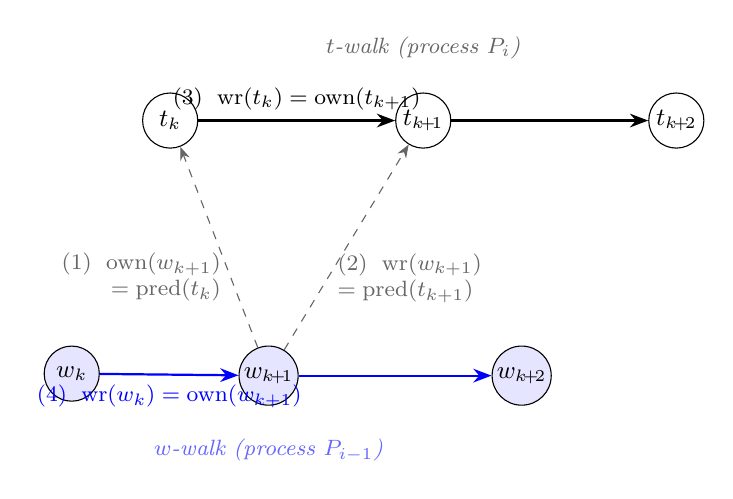
\begin{tikzpicture}[
    >=Stealth,
    every node/.style={font=\small},
    tnode/.style={draw, circle, minimum size=0.7cm, inner sep=1pt},
    wnode/.style={draw, circle, minimum size=0.7cm, inner sep=1pt, fill=blue!10},
]
  % t-walk (top row)
  \node[tnode] (t0) {$t_k$};
  \node[tnode, right=2.5cm of t0] (t1) {$t_{k\!+\!1}$};
  \node[tnode, right=2.5cm of t1] (t2) {$t_{k\!+\!2}$};
  \draw[->, thick] (t0) -- node[above, font=\footnotesize] {(3)\; $\operatorname{wr}(t_k) = \operatorname{own}(t_{k+1})$} (t1);
  \draw[->, thick] (t1) -- (t2);
  \node[above=0.3cm of t1, font=\footnotesize\itshape, text=black!60] {$t$-walk (process $P_i$)};

  % w-walk (bottom row)
  \node[wnode, below=2.5cm of t0, xshift=-1.25cm] (w0) {$w_k$};
  \node[wnode, below=2.5cm of t0, xshift=1.25cm] (w1) {$w_{k\!+\!1}$};
  \node[wnode, below=2.5cm of t1, xshift=1.25cm] (w2) {$w_{k\!+\!2}$};
  \draw[->, thick, blue] (w0) -- node[below, font=\footnotesize, text=blue] {(4)\; $\operatorname{wr}(w_k) = \operatorname{own}(w_{k+1})$} (w1);
  \draw[->, thick, blue] (w1) -- (w2);
  \node[below=0.3cm of w1, font=\footnotesize\itshape, text=blue!60] {$w$-walk (process $P_{i-1}$)};

  % Zigzag connections
  \draw[->, dashed, black!60] (w1) -- node[left, font=\footnotesize, pos=0.35, align=right] {(1)\; $\operatorname{own}(w_{k+1})$\\$= \operatorname{pred}(t_k)$} (t0);
  \draw[->, dashed, black!60] (w1) -- node[right, font=\footnotesize, pos=0.35, align=left] {(2)\; $\operatorname{wr}(w_{k+1})$\\$= \operatorname{pred}(t_{k+1})$} (t1);
\end{tikzpicture}
\caption{The zigzag coupling. The connecting witness $w_{k+1}$ sits between $t_k$ and $t_{k+1}$, linking them through its pre-fire state (condition~1) and written value (condition~2). Conditions (3) and (4) are H-edges within each walk.}
\label{fig:zigzag}
\end{figure}

\begin{remark}[Emergent shadow witness]
Conditions (1) and (2) together show that $w_{k+1}$ witnesses the shadow $\sigma(t_k, t_{k+1})$: $\operatorname{own}(w_{k+1}) = \operatorname{pred}(t_k)$ and $\operatorname{wr}(w_{k+1}) = \operatorname{pred}(t_{k+1})$. The shadow witness emerges directly from the zigzag structure. Combining conditions (1) and (4) gives $\operatorname{wr}(w_k) = \operatorname{pred}(t_k)$, which serves as the node condition for the product graph.
\end{remark}

\subsection{Construction}

\begin{definition}[Product transition graph]
\label{def:product}
Given a transition set $T$, the \emph{product transition graph} $G_\times(T)$ is defined as follows.

\textbf{Nodes:} Pairs $(t, w) \in T \times T$ such that $\operatorname{wr}(w) = \operatorname{pred}(t)$.

\textbf{Edges:} $(t_k, w_k) \to (t_{k+1}, w_{k+1})$ if all four equivariance conditions hold.

The product graph is built \emph{once} from $T$ and is not reconstructed during the algorithm.
\end{definition}

\begin{proposition}[Size]
$G_\times(T)$ has at most $|T|^2$ nodes and at most $|T|^4$ edges.
\end{proposition}

\subsection{Backward Propagation}

A cycle in $G_\times(T)$ encodes the coupling between two adjacent processes. In a ring, this coupling extends to all $K$ processes through \emph{backward propagation}: the $w$-walk of one coupling becomes the $t$-walk of the predecessor's coupling. The product graph captures this structure internally: if an arc has $w$-pair $(w_1, w_2)$, the predecessor coupling requires an arc with $t$-pair $(w_1, w_2)$---which is another arc in the \emph{same} product graph.

This observation motivates the three pruning operations in the algorithm.

%% ============================================================
\section{Livelock Analysis via the Product Graph}
\label{sec:bounded}
%% ============================================================

We develop the analysis through three subsections: the product graph's role in capturing equivariant walks, the witness-closed property, and the necessary/sufficient conditions for livelocks.

\subsection{The Product Graph Captures Pairwise Equivariant Walks}

By Definition~\ref{def:product}, a cycle in an equivariance graph $G_\times(S)$ is precisely a pair of closed walks---the $t$-walk and the $w$-walk---coupled by the four equivariance conditions at every step. A cycle of length $N$ in $G_\times(S)$ returns to its starting node $(t_0, w_0)$, so both the $t$-walk and the $w$-walk close with the same length $N$ by the graph structure.

Conversely, any pair of equivariant closed walks of the same length $N$ over $S$ defines a cycle of length $N$ in $G_\times(S)$. The product graph is a faithful representation of pairwise equivariant closed walks---it imposes no conditions beyond equivariance.

\begin{remark}[Self-disabling and the zigzag]
The product graph's faithfulness depends critically on self-disabling. In a self-disabling protocol, a process cannot fire again until its predecessor changes state. The coupling between adjacent processes is therefore one-to-one: each step of the $t$-walk corresponds to exactly one connecting witness in the $w$-walk, producing the zigzag $\ldots w_k \to t_k \to w_{k+1} \to t_{k+1} \to \ldots$ Without self-disabling, a process could fire multiple times between consecutive predecessor firings, the coupling would no longer be one-to-one, and the product graph would not faithfully capture the equivariant structure.

This one-to-one coupling is the token propagation discipline identified by Farahat and Ebnenasir~\cite{farahat-icdcs2012}: in a self-disabling ring, an enabled process fires, disables itself, and enables its successor---propagating the token forward without duplication or destruction. The zigzag is the algebraic expression of this discipline.
\end{remark}

The use of pairs is not incidental, and the reason is subtle. Given a closed $t$-cycle of period $N$, equivariance determines the predecessor's $\operatorname{own}$ and $\operatorname{wr}$ values at every position: the predecessor's H-walk is forced and closes automatically. However, the predecessor's $\operatorname{pred}$ values---which select which specific \emph{transitions} from $T$ realize the H-walk---are not determined by the $t$-cycle alone. In a non-deterministic protocol, multiple transitions may share the same $(\operatorname{own}, \operatorname{wr})$ but have different $\operatorname{pred}$ values. Different $\operatorname{pred}$ assignments yield different transition walks, which may close at different periods or not at all (see Section~\ref{sec:experiments}, Trial~56). This is the period determination problem: the $t$-cycle determines the predecessor's H-walk (a sequence of $\operatorname{own}/\operatorname{wr}$ values), but not its transition walk (a sequence of specific transitions from $T$).

The product graph resolves this by committing to specific transitions at every position---including their $\operatorname{pred}$ values. A cycle in the product graph returns to the \emph{same node} $(t_0, w_0)$, guaranteeing that the transition walk closes exactly, not just the H-walk. Pairs of transitions are the minimal unit that resolves the period: once a transition cycle is paired with a specific witness cycle, the equivariant closing period is determined.

\subsection{Witness-Closed Subgraphs}

\begin{definition}[Witness-closed subgraph]
\label{def:witness-closed}
A subgraph $G \subseteq G_\times(T)$ is \emph{witness-closed} if it satisfies two properties:
\begin{enumerate}[nosep]
\item \textbf{Cyclicity:} $G$ is a union of strongly connected components---every arc lies on a cycle.
\item \textbf{Backward closure:} For every arc on a cycle with $w$-pair $(w_1, w_2)$, there exists an arc $(w_1, u) \to (w_2, v)$ on a cycle in $G$.
\end{enumerate}
\end{definition}

\subsection{Necessary Condition: Livelock $\Rightarrow$ Witness-Closed Subgraph}

\begin{theorem}[Necessary condition for livelock]
\label{thm:necessary}
If a self-disabling unidirectional ring protocol with transition set $T$ admits a livelock, then $G_\times(T)$ contains a non-empty witness-closed subgraph.
\end{theorem}

\begin{proof}
A livelock at ring size $K$ is a valid tiling of the $K \times N$ torus~\cite{klinkhamer-ebnenasir}. Each row $i$ is a closed walk $W^{(i)}$ of length $N$ in the H-graph, and adjacent rows satisfy the four equivariance conditions. Let $S$ be the set of all transitions appearing in the tiling, and consider $G_\times(S)$.

For each adjacent pair of rows $(W^{(i)}, W^{(i-1)})$: both are closed walks of length $N$ (by the torus structure). The pair defines a closed walk of length $N$ in $G_\times(S)$, whose arcs all lie on a cycle. This establishes cyclicity.

For backward closure: the $w$-walk of coupling $(P_i, P_{i-1})$ is $W^{(i-1)}$, which is exactly the $t$-walk of coupling $(P_{i-1}, P_{i-2})$. The torus wraps after $K$ steps inward, providing cycle-level backward closure. Since cycle-level backward closure trivially implies arc-level backward closure (each arc on a cycle $C$ has its $w$-pair as a $t$-pair on the backward walk $C'$), the subgraph is witness-closed.

The arcs from all $K$ couplings form a subgraph of $G_\times(T)$. This subgraph satisfies cyclicity and backward closure---it is a non-empty witness-closed subgraph.
\end{proof}

\begin{corollary}[Livelock-freedom verifier]
\label{cor:freedom}
If $G^*(T) = \emptyset$ (the maximal witness-closed subgraph is empty), then the protocol is livelock-free for all ring sizes.
\end{corollary}

\subsection{Sufficient Condition via Backtracking}

When $G^*(T) \neq \emptyset$, we cannot immediately conclude that a livelock exists. Arc-level backward closure guarantees that every arc has a backward arc on a cycle, but this does not guarantee that a \emph{closed walk} backward-propagates into a torus (see Remark~\ref{rem:gap}).

We resolve this through backtracking: for each simple cycle $C$ in $G^*$, backward-propagate through $G^*$ by searching for a cycle in $G^*$ whose $t$-walk equals $C$'s $w$-walk. If the backward chain closes (a walk repeats), the torus is constructed and a livelock is confirmed.

\begin{theorem}[Sufficient condition for livelock]
\label{thm:sufficient}
Let $C_0$ be a simple cycle in $G^*(T)$. If the backward chain $C_0, C_1, C_2, \ldots$ (where each $C_{k+1}$ is a closed walk in $G^*$ whose $t$-walk equals $C_k$'s $w$-walk) closes---i.e., $C_j$ is a rotation of $C_i$ for some $j > i$---then the protocol admits a livelock at ring size $K = j - i$ with local period $N = |C_0|$.
\end{theorem}

\begin{proof}
The segment $C_i, C_{i+1}, \ldots, C_{j-1}$ provides $K = j-i$ pairs of equivariant closed walks, each of length $N$, with each $w$-walk serving as the next $t$-walk, and the orbit closing by the repetition condition. This is a valid tiling of the $K \times N$ torus, constituting a livelock~\cite{klinkhamer-ebnenasir}.
\end{proof}

\begin{remark}[Termination of backtracking]
For each simple cycle of length $N \leq |T|^2$, the backward chain visits closed walks of length $N$ in $G^*$. There are finitely many such walks (bounded by $|G^*|^N$). The chain either closes (livelock found) or reaches a dead end (no backward walk exists in $G^*$) within finitely many steps.
\end{remark}

\begin{remark}[Arc-level vs.\ cycle-level backward closure]
\label{rem:gap}
Arc-level backward closure guarantees that every arc has a backward arc on a cycle. This does not imply that a closed walk backward-propagates to a closed walk. The semi-algorithm searches for closing backward chains by exploring all backward walks---simple and compound. It is necessarily incomplete for chains that require walks longer than the longest cycle in $G^*$, consistent with the $\Sigma^0_1$-completeness of livelock detection.
\end{remark}

%% ============================================================
\section{The Algorithm}
\label{sec:algorithm}
%% ============================================================

By Corollary~\ref{cor:freedom}, $G^*(T) = \emptyset$ implies livelock-freedom. We compute the maximal witness-closed subgraph, then apply backtracking verification when it is non-empty.

\begin{definition}[Maximal product graph]
\label{def:maximal-product}
The \emph{maximal product graph} $G^*(T)$ is the largest witness-closed subgraph of $G_\times(T)$. Its \emph{support} is $L^* = \{t \in T : t \text{ appears in some node of } G^*(T)\}$.
\end{definition}

\begin{remark}[Uniqueness]
$G^*(T)$ is well-defined and unique: the witness-closed property is closed under union of arc sets (the union of two witness-closed subgraphs is witness-closed), so the maximal such subgraph exists. A non-empty witness-closed subgraph exists if and only if $G^*(T) \neq \emptyset$, since $G^*(T)$ contains every witness-closed subgraph.
\end{remark}

The algorithm computes $G^*(T)$ by building $G_\times(T)$ and iteratively pruning arcs that violate cyclicity or backward closure, until the fixed point is reached.

\begin{algorithm}[ht]
\caption{Computing the Maximal Product Graph $G^*(T)$}
\label{alg:main}
\begin{algorithmic}[1]
\Require Transition set $T$ (symmetric protocol)
\Ensure \textsc{Livelock-Free}, \textsc{Livelock}, or \textsc{Inconclusive}
\State Build full equivariance graph $G_\times(T)$ (Definition~\ref{def:product})
\Repeat
    \State \textbf{SCC:} Remove all arcs not on a cycle \Comment{enforce cyclicity}
    \State $S_t \gets \{\tau : (\tau, w) \text{ is on a cycle for some } w\}$ \Comment{$t$-components}
    \State \textbf{Square:} Remove arcs where $w_k \notin S_t$ or $w_{k+1} \notin S_t$
    \State \textbf{Backward:} For each surviving arc with $w$-pair $(w_1, w_2)$:
    \Statex \hspace{3.5em} if no arc $(w_1, u) \to (w_2, v)$ exists in $G_\times$ with $u, v \in S_t$, remove the arc
    \Statex \hspace{3.5em} \Comment{enforce backward closure}
\Until{no arcs removed}
\If{surviving arcs remain}
    \For{each simple cycle $C$ in the surviving graph}
        \State Backward-propagate $C$ through $G^*$: find closed walks in $G^*$
        \Statex \hspace{3.5em} whose $t$-walk matches $C$'s $w$-walk, iteratively
        \If{the backward chain closes (a walk repeats)}
            \State \Return \textsc{Livelock}
        \EndIf
    \EndFor
    \State \Return \textsc{Inconclusive} \Comment{$G^* \neq \emptyset$ but no cycle closes}
\Else
    \State \Return \textsc{Livelock-Free} \Comment{$G^*(T) = \emptyset$}
\EndIf
\end{algorithmic}
\end{algorithm}

\medskip

The algorithm enforces the two witness-closed properties through three pruning operations:
\begin{itemize}[nosep]
\item \textbf{SCC} enforces cyclicity by removing arcs not on any cycle.
\item \textbf{Square} is an auxiliary step that extracts $S_t$---the set of transitions appearing as $t$-components on cycles---and removes arcs whose $w$-components are not in $S_t$. This is implied by backward closure (if $(w_1, u) \to (w_2, v)$ is on a cycle, then $w_1$ and $w_2$ appear as $t$-components), but computing it explicitly provides the $S_t$ set needed by the backward closure check and accelerates convergence.
\item \textbf{Backward closure} checks each surviving arc's $w$-pair $(w_1, w_2)$: does $G_\times$ contain an arc $(w_1, u) \to (w_2, v)$ with $u, v \in S_t$?
\end{itemize}

The iteration is monotone (arcs are only removed) and operates on a finite set, so it terminates.

\begin{theorem}[Algorithm correctness]
\label{thm:algo-correctness}
Algorithm~\ref{alg:main} computes $G^*(T)$.
\end{theorem}

\begin{proof}
\textbf{Soundness} (the output is witness-closed). At the fixed point, no further arcs can be removed. The surviving arcs form a union of SCCs (by the SCC step), and every arc on a cycle has a backward arc on a cycle (by the backward closure step). Therefore the output satisfies cyclicity and backward closure.

\textbf{Completeness} (the output is maximal). We show that no arc of any witness-closed subgraph is ever removed. Let $G$ be any witness-closed subgraph, and consider any arc $e$ in $G$. It lies on a cycle in $G$ (by cyclicity), so SCC does not remove it. Its $w$-components appear as $t$-components on cycles in $G$ (by backward closure of $G$), so the square step does not remove it. Its $w$-pair has a backward arc on a cycle in $G$ (by backward closure of $G$), and these arcs also survive (by the same argument, inductively), so the backward closure step does not remove it. Therefore $G \subseteq \text{output}$ for every witness-closed subgraph $G$, and in particular $G^*(T) \subseteq \text{output}$. Combined with soundness, $\text{output} = G^*(T)$.
\end{proof}

\begin{corollary}[Soundness]
The algorithm is sound in both definitive directions. \textsc{Livelock-Free} is correct: $G^*(T) = \emptyset$ implies no livelock exists (Theorem~\ref{thm:necessary}). \textsc{Livelock} is correct: a closing backward chain constitutes a valid torus tiling (Theorem~\ref{thm:sufficient}). The \textsc{Inconclusive} outcome occurs when $G^* \neq \emptyset$ but no simple cycle's backward chain closes; this is consistent with livelock-freedom (as demonstrated by Kari's aperiodic tiles) or with livelock existence at a period beyond $|T|^2$.
\end{corollary}

\begin{theorem}[Complexity]
Phase~1 (computing $G^*(T)$) terminates in at most $O(|T|^4)$ iterations, each running in $O(|T|^4)$ time. Total: $O(|T|^8)$ worst case. Phase~2 (backtracking) is bounded: for each simple cycle of length $N \leq |T|^2$, the backward chain visits at most $|T|^{2N}$ distinct closed walks before repeating or dying. The total backtracking computation is finite but not polynomial.
\end{theorem}

\begin{proof}
Phase~1: the product graph has $O(|T|^4)$ arcs. Each iteration removes at least one arc. SCC and the pruning checks are linear in the number of arcs. Phase~2: the backward chain for a cycle of length $N$ visits closed walks of length $N$ in a graph of at most $|T|^2$ nodes. The number of distinct walks is finite (at most $|T|^{2N}$), so the chain terminates.
\end{proof}

\begin{remark}[Practical complexity]
For self-disabling protocols, $|T| = O(m^2)$.

This significantly improves the practical bounds. In the product graph, a node $(t, w)$ requires $\operatorname{wr}(w) = \operatorname{pred}(t)$; for a fixed $t$, there are $O(|T|/m)$ valid witnesses $w$. The product graph therefore has $O(|T|^2/m) = O(m^3)$ nodes and $O(|T|^4/m^3) = O(m^5)$ arcs. Each iteration costs $O(m^5)$ for SCC computation.

In practice, convergence occurs in very few iterations---at most 6 across all 4{,}349 protocols tested with $m$ up to 15---giving practical running time of $O(m^5)$. Pre-pruning $T$ by removing transitions not on any H-cycle (an $O(m^4)$ step) further reduces the product graph size, often dramatically.
\end{remark}

\begin{remark}[Necessity of the product graph]
A simpler algorithm operating directly on transitions and shadows---checking that each H-edge's shadow has an individual witness, without enforcing walk coherence---runs in $O(m^4)$ and is complete (never misses a livelock). However, it produces false positives: across 2{,}215 test protocols, it disagreed with the product graph on 55 cases (2.5\%), reporting livelocks where none exist. The product graph eliminates these false positives by enforcing that witnesses form coherent closed walks, not merely that individual shadows are witnessable. The $O(m^5)$ practical cost of the product graph is the price of soundness.
\end{remark}

\begin{remark}[$G^* = \emptyset$ and non-tileability]
\label{rem:non-tile}
The livelock-freedom guarantee from $G^*(T) = \emptyset$ may extend beyond periodic tileability. We conjecture that $G^*(T) = \emptyset$ implies the corresponding tile set cannot tile the infinite plane at all---not merely that no periodic tiling exists.

\emph{Proof sketch.} Consider any infinite tiling. At any two adjacent rows, the tiling defines a bi-infinite equivariant walk in $G_\times(T)$. Since $G_\times(T)$ is finite (at most $|T|^2$ nodes), every node visited by the bi-infinite walk is \emph{recurrent}---visited infinitely often in both directions. Every arc between recurrent nodes lies on a cycle (the walk departs and returns infinitely often). The tiling provides, at the next level, a bi-infinite equivariant walk whose arcs serve as backward arcs for the first level; these are also recurrent by the same argument. The union of all recurrent arcs across all adjacent row-pairs is a finite subset of $G_\times(T)$ satisfying cyclicity and backward closure---a non-empty witness-closed subgraph. Therefore $G^* \neq \emptyset$.

Contrapositively: $G^*(T) = \emptyset$ implies the tile set cannot tile the infinite plane. This is strictly stronger than ``no livelock.'' Note that this does \emph{not} contradict the undecidability of the domino problem~\cite{wang-tiles,berger}: $G^* = \emptyset$ is a sufficient condition for non-tileability, not a necessary one. Tile sets that cannot tile the plane may still have $G^* \neq \emptyset$ (local equivariant structure that does not extend globally). The domino problem remains undecidable because $G^* \neq \emptyset$ is inconclusive. Table~\ref{tab:landscape} summarizes the computability landscape.
\end{remark}

\begin{table}[ht]
\centering
\caption{Computability landscape for self-disabling tile sets. Non-tileability is $\Sigma^0_1$ (recognizable by patch enumeration); periodic tileability is $\Sigma^0_1$ (recognizable by torus enumeration); aperiodic tileability is in $\Pi^0_1$ (neither recognizer halts).}
\label{tab:landscape}
\smallskip
\begin{tabular}{l|ccc}
\hline
 & \textbf{Non-tileable} & \textbf{Aperiodic} & \textbf{Periodic} \\
\hline
$G^* = \emptyset$ & \checkmark (poly-time) & impossible$^*$ & impossible \\
Cycle closes & impossible & impossible & $N \leq |T|^2$ \\
\textsc{Inconclusive} & possible & Kari & $N > |T|^2$ \\
\hline
PROP & never halts & never halts & halts \\
\hline
\multicolumn{4}{l}{\footnotesize $^*$Conditional on Remark~\ref{rem:non-tile}.}
\end{tabular}
\end{table}

%% ============================================================
%% ============================================================
\section{Experimental Validation}
\label{sec:experiments}
%% ============================================================

The algorithm and all test protocols are available at\\ \url{https://github.com/cosmoparadox/mathematical-tools}.

\subsection{Known Protocols}

Algorithm~\ref{alg:main} correctly identifies:
\begin{itemize}[nosep]
\item \textbf{Dijkstra's token ring} ($(1,1)$-asymmetric, $m = 3, 4, 5$): livelock, forward shift 1.
\item \textbf{$3$-Coloring} (symmetric, $m = 3$): livelock, $e \equiv K \bmod 3$.
\item \textbf{Sum-Not-2} (symmetric, $m = 3$): livelock-free.
\item \textbf{Gouda--Haddix TB} (symmetric, $m = 8$): livelock, 14 surviving transitions out of 32, multiple livelock classes.
\end{itemize}

\subsection{Randomized Stress Testing}

We generated over 4{,}300 random self-disabling protocols across six categories: random seeds with $m \in \{3, \ldots, 10\}$, very dense protocols (near-complete transition sets), very sparse protocols ($m$ to $2m$ transitions), structured adversarial (coloring and agreement variants with noise), large domain sizes $m \in \{11, \ldots, 15\}$ with targeted density, and compound-witness-like protocols (large $m$, few transitions). Transition counts ranged from 3 to 120.

For each protocol, we computed $L^*$ via Algorithm~\ref{alg:main} and cross-checked against exhaustive state-space search at small ring sizes ($K \leq 6$).

\textbf{Results:} Zero false positives. Zero false negatives across all 4{,}349 protocols tested. The algorithm converged in at most 6 iterations in every case.

\subsection{Adversarial Protocols}

Randomized testing exposed a protocol ($m = 8$, 13 transitions) where a prior approach based on individual shadow checking produced a false positive: every shadow had a witness, but no \emph{coherent} witness walk existed. Shadow $(6, 5)$ was the bottleneck: no transition in $T$ has $\operatorname{own} = 6$, $\operatorname{wr} = 5$. The product graph correctly identifies this protocol as livelock-free, demonstrating the necessity of the product graph over local shadow-by-shadow analysis.

\subsection{K\&E Adversarial Protocol}

As a test of the product graph's faithfulness on structured adversarial inputs, we analyzed a protocol derived from Klinkhamer and Ebnenasir's SE tiling construction~\cite{klinkhamer-tr}: a symmetric self-disabling protocol with $m = 15$ and $|T| = 17$ transitions designed to exhibit complex livelock behavior. The product graph converges in a single iteration with all 17 transitions surviving ($|L^*| = 17$). Backtracking confirms the livelock: a simple cycle of length 6 backward-closes at depth 6.

\subsection{Kari's Aperiodic Tiles}

As the most stringent test of our semi-algorithm, we applied Klinkhamer and Ebnenasir's Lemma~4.8 gadget~\cite{klinkhamer-tr} to Kari's 14-tile aperiodic Wang tile set~\cite{kari-aperiodic}. Kari proved that these tiles tile the plane but admit no doubly-periodic tiling. The gadget converts the 14 tiles to a 54-transition self-disabling protocol with $m = 24$.

The algorithm produces $G^* \neq \emptyset$: 272 arcs survive the fixed-point pruning, with all 54 transitions in $L^*$. However, the backtracking phase examines over 5{,}000 simple cycles and finds that \emph{every} backward chain dies---no cycle closes. The algorithm reports \textsc{Inconclusive}, consistent with Kari's aperiodicity proof: no periodic tiling exists, so no livelock exists at any period.

This demonstrates the gap between arc-level and cycle-level backward closure (Remark~\ref{rem:gap}): the arc-level structure of $G^*$ admits rich cycle structure, but simple-cycle backward propagation correctly rejects every candidate. Compound closing chains---which exist for certain tile-theoretic constructions (Section~\ref{sec:counterexample})---are not searched. The semi-algorithm correctly returns \textsc{Inconclusive}, which is the expected outcome for an aperiodic tile set with no livelock. Across all 4{,}349 protocols tested---including protocols designed for self-stabilization, random protocols, and Wang tile gadgets---the \textsc{Free} and \textsc{Livelock} outcomes have never been wrong.

%% ============================================================
\section{Discussion}
\label{sec:discussion}
%% ============================================================

\subsection{Simple-Cycle Topology Preservation}

\begin{remark}[Simple and compound walks in closing chains]
\label{rem:walk-topology}
The backward propagation of cycles through $G^*$ may produce walks that are either simple (all positions visit distinct product graph nodes) or compound (some node visited at multiple positions). A closing backward chain can contain a mixture of both: a simple cycle may backward-propagate to a compound cycle and vice versa. The semi-algorithm explores all backward walks---simple and compound---without pruning.
\end{remark}


\subsection{Compound-Only Closing Chains: A Counterexample}
\label{sec:counterexample}

We demonstrate that livelocks can exist through compound closing chains in which no simple cycle backward-closes. This shows that the simple-cycle search is necessarily incomplete.

\paragraph{Construction.} Consider a $k$-bit forced binary counter encoded as NW-deterministic Wang tiles. For $k = 6$: each bit position $i \in \{0, \ldots, 5\}$ has four tiles encoding the half-adder logic $b' = b \oplus c$, $c' = b \wedge c$, where $b$ is the current bit, $c$ the carry-in, $b'$ the new bit, and $c'$ the carry-out. At position $k-1$, the carry-out is \emph{forced} to~1 regardless of the actual computation, ensuring carry is always injected at position~0. This eliminates degenerate (non-counting) tilings: 24 NW-deterministic tiles, period $2^6 = 64$. The Wang tiles (encoded as integer quadruples $(W, N, S, E)$) are:
{\small
\begin{align*}
\{&(12,0,0,13),\;(18,0,6,13),\;(12,6,6,13),\;(18,6,0,19),\\
  &(13,1,1,14),\;(19,1,7,14),\;(13,7,7,14),\;(19,7,1,20),\\
  &(14,2,2,15),\;(20,2,8,15),\;(14,8,8,15),\;(20,8,2,21),\\
  &(15,3,3,16),\;(21,3,9,16),\;(15,9,9,16),\;(21,9,3,22),\\
  &(16,4,4,17),\;(22,4,10,17),\;(16,10,10,17),\;(22,10,4,23),\\
  &(17,5,5,18),\;(23,5,11,18),\;(17,11,11,18),\;(23,11,5,18)\}.
\end{align*}
}

\paragraph{Through the K\&E gadget.} The 24 tiles produce an 89-transition self-disabling protocol with $m = 73$. The gadget's $2 \times 2$ block structure yields an action-tile torus of $128 \times 12$, corresponding to a livelock with ring size $K = 12$ and local period $N = 128$. The protocol is available as the \texttt{forced\_counter} example in the accompanying tool.

\paragraph{Algorithm result.} For $k = 6$: $G^*$ retains 82 transitions and 146 arcs. The semi-algorithm discovers 39 simple cycles and explores compound walks through backward propagation, reaching 92 canonical cycles total. None close. The semi-algorithm returns \textsc{Inconclusive} because the livelock period ($N = 128$) exceeds the longest cycle discoverable from the product graph's simple cycles (length~12). For $k = 2$ (period~4), the semi-algorithm successfully detects the livelock through a closing chain that includes both simple and compound walks, demonstrating that compound backward propagation is essential.

\paragraph{Verified livelock.} The livelock is verified by direct construction: 12 process walks of length 128, each forming a valid H-walk, with equivariant coupling between adjacent processes confirmed at all 128 time steps.

\paragraph{Compound closing chain.} The 12 process-pair walks map into $G^*$ as compound walks (4 to 14 distinct product graph nodes out of 128 positions). All nodes and arcs lie in $G^*$. Each backward step is verified: $t$-component matches $w$-component of the source, arcs exist in $G^*$, and the walk closes. The chain closes at depth~12.

\paragraph{Topology breaking.} The backward maps are \emph{not} bijections on nodes. The distinct node counts across the closing chain are:
\[
4 \to 10 \to 8 \to 14 \to 8 \to 14 \to 8 \to 14 \to 8 \to 14 \to 8 \to 8 \to 4.
\]
The map from 4 distinct nodes to 10 distinct nodes cannot be a bijection on nodes. The backward map is single-valued on \emph{positions} (the identity) but multi-valued on \emph{nodes}: a node appearing at positions $a$ and $b$ maps to different targets depending on position context. This position-versus-node gap is characteristic of compound closing chains and is the source of the semi-algorithm's incompleteness when walk lengths exceed the product graph's simple cycle capacity.

\subsection{Empirical Evidence on Natural Protocols}

Despite the existence of the forced-counter counterexample, the semi-algorithm produces correct \textsc{Free} and \textsc{Livelock} outcomes on all protocols designed for self-stabilization. Table~\ref{tab:evidence} summarizes the results.

\begin{table}[ht]
\centering
\caption{Empirical results on protocols designed for self-stabilization. Across all experiments, every protocol admitting a livelock is conclusively identified. The \textsc{Inconclusive} outcome occurs only on Kari's aperiodic tiles and the forced binary counter.}
\label{tab:evidence}
\smallskip
\begin{tabular}{lrrr}
\hline
\textbf{Experiment} & \textbf{Count} & \textbf{Conclusive} & \textbf{Errors} \\
\hline
Self-disabling protocols (random) & 4{,}349 & 4{,}349 & 0 \\
Non-self-disabling (augmented) & 6{,}000+ & 6{,}000+ & 0 \\
Wang tile gadgets (NW-det, random) & 500+ & 500+ & 0 \\
K\&E adversarial + Kari aperiodic & 2 & 2 & 0 \\
NW-det Mealy machines ($c \leq 4$) & 10{,}000+ & 10{,}000+ & 0 \\
\hline
\textbf{Total} & \textbf{21{,}000+} & \textbf{21{,}000+} & \textbf{0} \\
\hline
\end{tabular}
\end{table}

\paragraph{No protocol designed for self-stabilization exhibits compound-only closure.} Across 278 confirmed livelocks from protocols designed for self-stabilization, every closing chain consists entirely of simple cycles. No protocol designed for self-stabilization---including adversarial constructions from K\&E---has ever produced a compound-only closing chain. The forced binary counter is the only construction we have found that exhibits this structure, and it requires an explicit carry-forcing mechanism that does not arise in protocols designed for self-stabilization.

\paragraph{All-or-nothing property.} For protocols designed for self-stabilization, closure is a global property of $G^*$: either all simple cycles close (livelock exists) or none do (no livelock through simple cycles). No mixed pattern has been observed.

\subsection{Relationship to Undecidability}

Mazoyer and Rapaport~\cite{mazoyer-rapaport} proved that the NW-deterministic periodic domino problem is undecidable, by reduction from the Turing machine halting problem. Klinkhamer and Ebnenasir~\cite{klinkhamer-ebnenasir} showed this implies $\Sigma^0_1$-completeness of livelock detection for self-disabling protocols.

Our counterexample is consistent with this undecidability. The forced binary counter encodes a modular counting structure whose period grows exponentially ($2^k$) while the tile count grows linearly ($4k$). Through the K\&E gadget, the livelock exists at period $N = 2 \cdot 2^k$ within a product graph of $O(k^2)$ nodes. For sufficiently large $k$, the livelock period exceeds $|T|^2$, and the closing chain is necessarily compound. The semi-algorithm, which searches only simple cycles, cannot detect it.

More broadly, Mazoyer and Rapaport's construction embeds Turing machine computations in hierarchical Robinson-tile structures, producing NW-deterministic tile sets with unbounded minimum periods. These map through the K\&E gadget to protocols whose livelocks have compound-only closing chains of unbounded depth. The simple-cycle search is sound but incomplete, and no finite extension can make it complete.

\paragraph{What the semi-algorithm decides.} The semi-algorithm decides livelock detection for the class of protocols whose livelocks (if any) have simple closing chains. This class includes all 21{,}000+ protocols we have tested, none of which were designed to encode computation. The undecidable cases---those with compound-only closing chains---arise exclusively from tile-theoretic constructions encoding computation, and have not been observed in any protocol designed for self-stabilization.

\subsection{Iterated Product Graphs}

The product graph $G_\times(T)$ captures pairwise equivariance between two adjacent rows of the torus. An \emph{iterated} product graph $G_\times^{(n)}(T)$, constructed by taking the product graph of $G_\times^{(n-1)}(T)$ with the original transition graph, captures equivariance across $n+1$ adjacent rows simultaneously.

A compound walk in $G_\times^{(1)}$---one that revisits product graph nodes---may become a \emph{simple} walk in $G_\times^{(n)}$ for sufficiently large $n$, because the additional row context disambiguates the repeated positions. For instance, a walk visiting 4 distinct nodes at 128 positions in $G_\times^{(1)}$ might visit 128 distinct nodes in $G_\times^{(n)}$, where the extended context distinguishes each occurrence. Once the walk is simple in $G_\times^{(n)}$, the backward propagation search at level $n$ explores a richer space of walks and can detect livelocks that were invisible at lower levels.

Each iteration increases the state space from $O(|T|^{2n})$ to $O(|T|^{2(n+1)})$, raising the computational cost but strictly increasing the class of detectable livelocks. This provides a tower of increasingly powerful semi-decision procedures:
\[
G_\times^{(1)}(T) \subset G_\times^{(2)}(T) \subset \cdots
\]
For any fixed protocol with a livelock of period $N$, there exists a level $n$ at which the livelock's walk becomes simple in $G_\times^{(n)}$ and the semi-algorithm detects it. Similarly, non-tileable instances are caught by $G^* = \emptyset$ at some finite level. The tower thus terminates with a definitive answer (\textsc{Free} or \textsc{Livelock}) for every non-aperiodic instance. The undecidability manifests exclusively in aperiodic instances: $G^* \neq \emptyset$ at every level, no cycle ever closes, and the tower produces \textsc{Inconclusive} indefinitely. Distinguishing ``aperiodic, livelock-free'' from ``periodic with very large period'' is precisely where $\Sigma^0_1$-completeness resides.

%% ============================================================
\section{Extension to Non-Self-Disabling Protocols}
\label{sec:non-sd}
%% ============================================================

The product graph and the theory of equivariant walks assume self-disabling protocols, where firing a transition disables it until the predecessor changes value. Many practical protocols violate this constraint: under a fixed predecessor value, a process may fire a sequence of transitions---a \emph{burst}---before the predecessor acts. We show that a simple protocol transformation reduces the non-self-disabling case to the self-disabling framework.

\subsection{Protocol Transformation}

\begin{definition}[Burst closure]
\label{def:burst}
For a transition set $T$ and a predecessor value $p$, define the \emph{chain graph} $C_p$ as the directed graph on domain values with edge $o \to w$ for each $(p, o, w) \in T$. The \emph{burst closure} $\hat{T}$ is:
\[
\hat{T} = T \cup \{(p, o, w') : w' \text{ is reachable from } o \text{ in } C_p,\; o \neq w'\}
\]
\end{definition}

The burst closure adds, for each predecessor value $p$, all transitions $(p, o_i, o_j)$ where $o_j$ is reachable from $o_i$ via any chain of transitions under the same predecessor. These macro-transitions represent the net effect of a process firing multiple transitions in succession while its predecessor's value remains $p$.

\begin{proposition}[Local cycle detection]
If $C_p$ contains a directed cycle for any predecessor value $p$, then the protocol admits a trivial livelock: a process can fire transitions indefinitely under fixed predecessor value $p$.
\end{proposition}

\subsection{Correspondence}

\begin{theorem}[Execution-walk correspondence]
\label{thm:burst-correspondence}
Let $T$ be an arbitrary (possibly non-self-disabling) transition set for a unidirectional ring protocol, and let $\hat{T}$ be its burst closure with no local cycles. Then:
\begin{enumerate}[nosep]
\item Every livelock of the protocol under $T$ corresponds to an equivariant closed walk in $G_\times(\hat{T})$.
\item Every equivariant closed walk in $G_\times(\hat{T})$ corresponds to a valid execution of the protocol under $T$.
\end{enumerate}
\end{theorem}

\begin{proof}
\textbf{Direction 1.} In a livelock under $T$, each process $P_i$ executes a periodic sequence of transitions. Between consecutive changes of $P_{i-1}$'s value, process $P_i$ fires a burst of transitions under a fixed predecessor value $p$---a path in $C_p$ from some $o$ to some $w'$. The transition $(p, o, w') \in \hat{T}$ captures this burst as a single macro-transition. The sequence of macro-transitions at $P_i$ forms a closed walk in the H-graph of $\hat{T}$, and the equivariance between $P_i$'s macro-transitions and $P_{i-1}$'s macro-transitions is preserved because each macro-transition's predecessor value is $P_{i-1}$'s value \emph{at the start of the burst}---exactly the value written by $P_{i-1}$'s preceding macro-transition.

\textbf{Direction 2.} An equivariant closed walk in $G_\times(\hat{T})$ consists of macro-transitions $(p, o, w') \in \hat{T}$. Each macro-transition corresponds to a realizable path in the chain graph $C_p$: a sequence of original transitions $(p, o, o_1), (p, o_1, o_2), \ldots, (p, o_{k-1}, w')$ all in $T$. Since the predecessor value $p$ is fixed during the burst (the equivariance conditions ensure $P_{i-1}$ does not change value until $P_i$ completes its burst), this sequence is a valid execution segment. Concatenating the burst segments across all positions and all processes yields a valid execution under $T$.
\end{proof}

\begin{corollary}
The product graph algorithm applied to $\hat{T}$ is a sound livelock analyzer for arbitrary unidirectional ring protocols: $G^*(\hat{T}) = \emptyset$ implies the protocol under $T$ is livelock-free for all ring sizes.
\end{corollary}

The burst closure $\hat{T}$ is generally \emph{not} self-disabling---it retains transitions $(p, o_1, o_2)$ and $(p, o_2, o_3)$ simultaneously. The product graph algorithm operates on $\hat{T}$ without modification: the four equivariance conditions, SCC pruning, and backward closure are purely graph-theoretic and do not require self-disabling.

%% ============================================================
\section{Extension to $(1,1)$-Asymmetric Protocols}
\label{sec:asymmetry}
%% ============================================================

For a $(1,1)$-asymmetric ring with transition sets $T_0$ (distinguished process $P_0$) and $T_o$ (all other processes), three product graphs capture the three coupling types:

\begin{enumerate}[nosep]
\item $G_1 = G_\times(T_o, T_0)$: predecessor fires $T_o$, successor fires $T_0$. The $P_o \to P_0$ coupling.
\item $G_2 = G_\times(T_0, T_o)$: predecessor fires $T_0$, successor fires $T_o$. The $P_0 \to P_o$ coupling.
\item $G_3 = G_\times(T_o, T_o)$: both fire $T_o$. The bulk $P_o \to P_o$ coupling.
\end{enumerate}

Each graph is built independently using the same four equivariance conditions.

\subsection{Cross-Graph Backward Closure}

In the symmetric case, the backward closure check verifies that each $w$-edge has a predecessor arc \emph{within the same product graph}. For asymmetric protocols, the predecessor coupling may reside in a \emph{different} product graph.

The three graphs form a ring of backward dependencies:
\[
G_1 \to G_3 \to G_3 \to \cdots \to G_3 \to G_2 \to G_1
\]
An arc in $G_1$ with $w$-pair $(w_1, w_2)$ requires a predecessor arc with $t$-pair $(w_1, w_2)$. Since the predecessor of $P_0$'s predecessor fires $T_o$, this predecessor arc lies in $G_3$, not $G_1$. Similarly, arcs in $G_2$ require predecessor arcs in $G_1$, and arcs in $G_3$ require predecessor arcs in either $G_3$ (bulk) or $G_2$ (at the boundary).

\subsection{Joint Algorithm}

The algorithm extends naturally: apply SCC, square, and backward closure to each graph, but the backward closure check references the \emph{appropriate neighboring graph} for the predecessor arc:

\begin{itemize}[nosep]
\item For $G_1$ ($P_o \to P_0$): backward closure checks predecessor arcs in $G_3$.
\item For $G_2$ ($P_0 \to P_o$): backward closure checks predecessor arcs in $G_1$.
\item For $G_3$ ($P_o \to P_o$): backward closure checks predecessor arcs in $G_3$ itself (and in $G_2$ for the boundary process).
\end{itemize}

The square support $S_t$ is computed per graph: $S_t^{(k)}$ is the set of $t$-components on cycles in $G_k$. The backward closure check for an arc in $G_k$ with $w$-pair $(w_1, w_2)$ verifies that the neighboring graph contains an arc $(w_1, u) \to (w_2, v)$ with $u, v \in S_t^{(\text{neighbor})}$.

Pruning in one graph may invalidate arcs in neighboring graphs through the cross-graph backward closure, triggering a cascade that propagates bidirectionally around the ring of graphs until quiescence.

\subsection{Termination and Correctness}

\begin{theorem}
The $(1,1)$-asymmetric algorithm terminates. Soundness: if all three graphs collapse to $\emptyset$, the protocol is livelock-free for all ring sizes. Completeness: every livelock maps into the three graphs as surviving arcs.
\end{theorem}

\begin{proof}
\textbf{Termination.} The total number of arcs across all three graphs is finite, each iteration removes at least one, and arcs are never re-added.

\textbf{Completeness.} A livelock provides explicit walks and couplings that form surviving arcs in each graph. The cross-graph backward closure is satisfied because adjacent processes' walks serve as each other's predecessor couplings.

\textbf{Soundness.} The arc-level backward closure is a necessary condition for livelocks (by completeness, every livelock produces surviving arcs). If all three graphs collapse to $\emptyset$, no livelock can exist. As in the symmetric case, non-empty surviving graphs require backtracking verification to confirm livelock existence.
\end{proof}

\begin{remark}
For general $(l,q)$-asymmetry, one product graph per distinct coupling type suffices, with backward closure checks referencing the appropriate neighbor in the coupling ring. We leave the full treatment to future work.
\end{remark}

%% ============================================================
\section{Related Work}
\label{sec:related}
%% ============================================================

\paragraph{Automata, tiling languages, and symbolic dynamics.} Our product graph can be viewed as a finite automaton for a restricted tiling language. In the Vardi--Wolper automata-theoretic approach to model checking~\cite{vardi-wolper}, a product automaton decides temporal properties by reducing them to cycle detection in a finite graph. Our construction follows the same pattern, but the ``language'' is a set of valid SE torus tilings under the self-disabling constraint, where each symbol is a transition--witness pair drawn from an alphabet of size $|T|^2$. The product graph is the automaton: its cycles are valid row-pairs, and backward closure is the self-referential constraint ensuring that the automaton's output (the $w$-walk) is itself accepted as input (the $t$-walk of the next row). This connects to symbolic dynamics~\cite{lind-marcus}: two-dimensional sofic shifts---sets of valid tilings---are generally undecidable (Wang~\cite{wang-tiles}, Berger~\cite{berger}). Self-disabling collapses the two-dimensional structure into a one-dimensional shift with a self-referential constraint (backward closure). The product graph provides a finite representation of this shift, enabling polynomial-time livelock-freedom verification.

\paragraph{Parameterized verification: general undecidability.} Apt and Kozen~\cite{apt-kozen} showed that verifying LTL properties for parameterized systems is $\Pi^0_1$-complete. Suzuki~\cite{suzuki} strengthened this to unidirectional rings. Esparza~\cite{esparza} surveys the complexity landscape of parameterized verification. These results establish the general barrier; our work identifies a structural regime where effective verification is possible, even if full decidability remains open.

\paragraph{Cutoff results.} Emerson and Namjoshi~\cite{emerson-namjoshi} introduced cutoff-based reasoning for rings: if a property holds for rings up to a cutoff size, it holds for all sizes. Emerson and Kahlon~\cite{emerson-kahlon} extended cutoffs to guarded protocols and ring-based message passing. These results reduce parameterized verification to finite model checking at a fixed size; our approach is complementary, reducing the problem to a fixed-point computation on the product graph independent of any specific ring size.

\paragraph{Well-quasi-orderings.} Abdulla et al.~\cite{abdulla-wqo} developed a general framework for infinite-state systems using well-quasi-orderings (WQOs): if states are well-quasi-ordered and transitions are monotonic, backward reachability terminates. Finkel and Schnoebelen~\cite{finkel-wsts} systematized this as the theory of well-structured transition systems (WSTSs). Our approach is different in mechanism---it arises from the bounded space of transition--witness pairs in the equivariant product, not from a WQO on states---but follows a similar pattern: lifting to a space where a structural property becomes explicit, enabling effective verification of livelock-freedom. Recent work extends WSTS techniques to threshold automata for round-based distributed algorithms~\cite{baumeister-jacobs}.

\paragraph{Tiling and undecidability.} Wang~\cite{wang-tiles} introduced the domino problem: does a given tile set tile the plane? Berger~\cite{berger} proved undecidability. The periodic variant---does the tile set admit a doubly-periodic tiling?---is also undecidable~\cite{gurevich-koryakov}. Kari~\cite{kari-aperiodic} proved that the general domino problem remains undecidable for NW-deterministic tile sets. Mazoyer and Rapaport~\cite{mazoyer-rapaport} proved that the \emph{periodic} domino problem is undecidable for NW-deterministic tile sets, by reduction from the Turing machine halting problem using Robinson's aperiodic hierarchy. Klinkhamer and Ebnenasir~\cite{klinkhamer-ebnenasir} reduce the NW-deterministic periodic domino problem to livelock detection via an SE (South=East) tiling gadget that enforces self-disabling. Our product graph provides a polynomial-time livelock-freedom verifier ($G^* = \emptyset$) and a sound livelock detector (backtracking over simple cycles). Consistent with Mazoyer and Rapaport's undecidability, we exhibit a concrete counterexample---a forced binary counter whose livelock exists only through compound closing chains (Section~\ref{sec:counterexample}).

\paragraph{Algebraic characterization and combinatorial lifting.} Farahat~\cite{farahat-diss} introduced an algebraic framework for livelock analysis in which livelocks are characterized by cyclic equivariance relations on the transition space---closed walks in the H-graph with compatible shadows. Farahat and Ebnenasir~\cite{farahat-icdcs2012} showed that the token-passing discipline induced by self-disabling enables local reasoning about global convergence properties. Klinkhamer and Ebnenasir~\cite{klinkhamer-ebnenasir} lifted Farahat's algebraic characterization to the combinatorial setting of torus tilings, establishing the equivalence between livelocks and doubly-periodic tilings of a $K \times N$ torus via the ``leads'' relation---which is precisely the equivariance coupling. Their torus characterization revealed the connection to the periodic domino problem, yielding $\Sigma^0_1$-completeness of livelock detection. Our product transition graph builds on their framework: it realizes the equivariance coupling as a finite automaton whose state space supports effective backward propagation search (Section~\ref{sec:discussion}).

\paragraph{Relationship to Klinkhamer and Ebnenasir's undecidability result and PROP.}
Their characterization~\cite{klinkhamer-ebnenasir} is correct and complete: a livelock exists if and only if $m$ periodic propagations of period $n$ exist, each leading the next. Their torus formulation revealed the connection to the periodic domino problem, yielding $\Sigma^0_1$-completeness for livelock detection and $\Pi^0_1$-completeness for livelock-freedom verification. Their semi-algorithm PROP~\cite{klinkhamer-tr} searches for propagations by incrementally increasing scope parameters $(m, n)$. PROP is sound: any reported livelock is genuine. However, PROP is a pure semi-decider for livelock existence ($\Sigma^0_1$): it can find livelocks but can never prove livelock-freedom---if no livelock exists, PROP runs indefinitely without reaching a conclusion.

Our semi-algorithm is strictly stronger in three respects. First, $G^*(T) = \emptyset$ proves livelock-freedom in polynomial time---a capability PROP entirely lacks. Second, our semi-algorithm always terminates with one of three outcomes (\textsc{Free}, \textsc{Livelock}, \textsc{Inconclusive}), whereas PROP may run indefinitely. The \textsc{Inconclusive} outcome is genuine: it correctly arises from aperiodic tile structures where no livelock exists (Kari) or from compound-only closing chains (forced binary counter, Section~\ref{sec:counterexample}). Across all 21{,}000+ protocols tested---including adversarial constructions from K\&E and protocols designed for self-stabilization---the \textsc{Free} and \textsc{Livelock} outcomes have never been incorrect.

\paragraph{Product constructions and finite abstractions.} Our approach instantiates a pattern recurring across verification and combinatorics: problems that appear unbounded in their native representation become tractable when lifted to a space where the governing invariant is explicit. The Myhill--Nerode theorem reduces language equivalence to a finite quotient; synchronized products in model checking compose automata to expose global reachability; symbolic dynamics~\cite{lind-marcus} lifts shift spaces to finite graphs of forbidden patterns. Our product transition graph plays an analogous role: it lifts equivariant transition walks to a bounded graph of transition--witness pairs, enabling efficient pruning of the search space.

\paragraph{Modern parameterized verification.} Recent approaches to parameterized verification and synthesis, including threshold automata~\cite{baumeister-jacobs}, SMT-based techniques~\cite{mirzaie-bonakdarpour}, and cutoff-based methods~\cite{bloem-survey}, face the same fundamental trade-off: decidable subclasses guarantee termination but restrict expressiveness, while semi-decision procedures handle broader classes but may diverge. Baumeister et al.~\cite{baumeister-jacobs} observe that in practice this line blurs---semi-decision procedures often terminate on the instances that arise in practice, effectively deciding fragments of their input space. Our work exemplifies this pattern: the semi-algorithm is incomplete in theory (consistent with $\Sigma^0_1$-completeness), but across 21{,}000+ protocols---including all known adversarial constructions from the self-stabilization literature---it has never failed to reach a definitive conclusion. What distinguishes our approach from typical semi-decision procedures is that it provides polynomial-time certificates in \emph{both} directions: $G^* = \emptyset$ certifies livelock-freedom (a $\Pi^0_1$ capability that pure semi-deciders like PROP lack), and closing cycles certify livelock existence.

%% ============================================================
\section{Conclusion}
\label{sec:conclusion}
%% ============================================================

We have developed a practical framework for livelock analysis in parameterized unidirectional rings, occupying the middle ground between decidable subclasses and pure semi-decision procedures in parameterized verification~\cite{bloem-survey}. The product transition graph $G^*(T)$ provides polynomial-time certificates in both directions: $G^* = \emptyset$ certifies livelock-freedom, and closing cycles certify livelock existence. The resulting semi-algorithm always terminates with one of three outcomes (\textsc{Free}, \textsc{Livelock}, \textsc{Inconclusive}), distinguishing it from PROP~\cite{klinkhamer-tr} which may run indefinitely.

The semi-algorithm is necessarily incomplete: a forced binary counter (Section~\ref{sec:counterexample}) produces a verified livelock that exists only through compound closing chains with topology-breaking backward maps, consistent with the $\Sigma^0_1$-completeness established by Mazoyer and Rapaport~\cite{mazoyer-rapaport}. The iterated product graph construction (Section~\ref{sec:discussion}) provides a principled path toward detecting such livelocks at higher computational cost.

Despite this theoretical limitation, across 21{,}000+ protocols the \textsc{Free} and \textsc{Livelock} outcomes have zero errors. No protocol designed for self-stabilization has ever produced the \textsc{Inconclusive} outcome.

\paragraph{Future directions.}
\begin{enumerate}[nosep]
\item \textbf{Characterizing compound-only protocols.} What structural properties force livelocks to exist only through compound closing chains? Understanding the full class would sharpen the semi-algorithm's scope guarantee.

\item \textbf{Non-tileability certificate.} Does $G^*(T) = \emptyset$ imply non-tileability for all self-disabling tile sets?

\item \textbf{$(l,q)$-asymmetry.} Extending the three-graph construction to arbitrary numbers of process types.
\end{enumerate}

%% ============================================================
%\section*{Acknowledgments}
%% ============================================================

%% ============================================================
\appendix
\section{Detailed Examples}
\label{sec:examples}
%% ============================================================

\subsection{$3$-Coloring (Symmetric, $m = 3$)}

$T = \{(0,0,1),\; (1,1,2),\; (2,2,0)\}$. All transitions survive. One simple cycle $c_0$ of length $N = 3$, self-enabling with forward shift $s = 1$.

\subsection{Dijkstra's Token Ring ($m = 3$, $(1,1)$-asymmetric)}

$T_0 = \{(0,0,1),\; (1,1,2),\; (2,2,0)\}$, $T_o = \{(0,2,0),\; (1,0,1),\; (2,1,2)\}$.

Three product graphs: $G_\times(T_o, T_0)$, $G_\times(T_0, T_o)$, $G_\times(T_o, T_o)$. Forward shift 1 in $T_0$, shift 0 in $T_o$.

\subsection{Compound Witness Protocol (Symmetric, $m = 16$)}

\begin{align*}
T = \{&(5,2,3),\; (8,3,2),\; (2,7,9),\; (3,9,12),\; (2,12,15),\\
      &(3,15,7),\; (7,5,8),\; (9,8,5),\; (12,5,8),\; (15,8,5)\}.
\end{align*}

All 10 transitions survive. Eight simple cycles in $H(T)$. The product graph detects a livelock with local period $N = 4$. This protocol demonstrates compound witness chains: the simple H-cycle of length 2 is a dead-end in the product graph, but a compound walk of length 4 (repeating the 2-cycle twice with different witnesses) is self-sustaining.

\subsection{Trial 56: Shadow Coherence Failure ($m = 8$)}

\begin{align*}
T = \{&(0,4,2),\; (0,7,6),\; (2,2,7),\; (2,5,7),\; (3,6,0),\; (4,0,2),\; (4,0,5),\\
      &(5,2,0),\; (5,6,0),\; (6,3,4),\; (6,6,2),\; (7,0,6),\; (7,7,3)\}.
\end{align*}

All 13 transitions lie on H-graph cycles. Of the 28 H-edges, 20 have individually witnessed shadows---only 8 lack witnesses. After removing those 8 edges, the remaining H-graph still contains cycles. A transition-level analysis (individual shadow checking) reports this protocol as a livelock.

However, no livelock exists. The unwitnessed shadows---including $(0,3)$, $(3,7)$, $(4,5)$, $(5,4)$, $(6,5)$, $(7,5)$---create gaps in the witness value space. Each H-cycle can find individual witnesses for its own shadows, but those witnesses form walks whose shadows hit the gaps. The incoherence manifests two levels deep in the witness chain.

The product graph $G_\times(T)$ starts with 42 arcs. Backward closure prunes 18 arcs in the first iteration; the surviving 24 arcs collapse to $\emptyset$ in the second (no remaining SCC). Result: livelock-free, confirmed by exhaustive state-space search at all ring sizes $K \leq 8$.

This protocol demonstrates that individual shadow witnessing is strictly weaker than the product graph's backward closure. The product graph detects that no coherent witness walk exists, even when individual shadows are witnessable.

%% ============================================================
\bibliographystyle{plain}
\begin{thebibliography}{10}

\bibitem{abdulla-wqo}
P.~A. Abdulla, K.~\v{C}er\={a}ns, B.~Jonsson, and Y.-K. Tsay.
\newblock Algorithmic analysis of programs with well quasi-ordered domains.
\newblock {\em Information and Computation}, 160(1--2):109--127, 2000.

\bibitem{apt-kozen}
K.~R. Apt and D.~Kozen.
\newblock Limits for automatic verification of finite-state concurrent systems.
\newblock {\em Information Processing Letters}, 22(6):307--309, 1986.

\bibitem{baumeister-jacobs}
T.~Baumeister, P.~Eichler, S.~Jacobs, M.~Sakr, and M.~V\"olp.
\newblock Parameterized verification of round-based distributed algorithms via extended threshold automata.
\newblock {\em arXiv preprint arXiv:2406.19880}, 2024.

\bibitem{bloem-survey}
R.~Bloem, S.~Jacobs, A.~Khalimov, I.~Konnov, S.~Rubin, H.~Veith, and J.~Widder.
\newblock Decidability of Parameterized Verification.
\newblock Synthesis Lectures on Distributed Computing Theory. Morgan \& Claypool, 2015.

\bibitem{berger}
R.~Berger.
\newblock The undecidability of the domino problem.
\newblock {\em Memoirs of the American Mathematical Society}, 66, 1966.

\bibitem{bloem-book}
R.~Bloem, S.~Jacobs, A.~Khalimov, I.~Konnov, S.~Rubin, H.~Veith, and J.~Widder.
\newblock {\em Decidability of Parameterized Verification}.
\newblock Synthesis Lectures on Distributed Computing Theory. Morgan \& Claypool, 2015.

\bibitem{dijkstra1974}
E.~W. Dijkstra.
\newblock Self-stabilizing systems in spite of distributed control.
\newblock {\em Communications of the ACM}, 17(11):643--644, 1974.

\bibitem{emerson-kahlon}
E.~A. Emerson and V.~Kahlon.
\newblock Parameterized model checking of ring-based message passing systems.
\newblock In {\em Proceedings of CSL}, LNCS 3210, pages 325--339. Springer, 2004.

\bibitem{emerson-namjoshi}
E.~A. Emerson and K.~S. Namjoshi.
\newblock On reasoning about rings.
\newblock {\em International Journal of Foundations of Computer Science}, 14(4):527--549, 2003.

\bibitem{esparza}
J.~Esparza.
\newblock Keeping a crowd safe: On the complexity of parameterized verification (invited talk).
\newblock In {\em STACS}, LIPIcs vol.~25, pages 1--10. Schloss Dagstuhl, 2014.

\bibitem{emerson-namjoshi}
E.~A. Emerson and K.~S. Namjoshi.
\newblock Reasoning about rings.
\newblock In {\em Proceedings of the 22nd ACM Symposium on Principles of Programming Languages (POPL)}, pages 85--94, 1995.

\bibitem{farahat-diss}
A.~Farahat.
\newblock {\em Automated Design of Self-Stabilization}.
\newblock PhD thesis, Michigan Technological University, 2012.

\bibitem{farahat-icdcs2012}
A.~Farahat and A.~Ebnenasir.
\newblock Local reasoning for global convergence of parameterized rings.
\newblock In {\em Proceedings of IEEE ICDCS}, pages 496--505, 2012.

\bibitem{finkel-wsts}
A.~Finkel and Ph.~Schnoebelen.
\newblock Well-structured transition systems everywhere!
\newblock {\em Theoretical Computer Science}, 256(1--2):63--92, 2001.

\bibitem{gouda-haddix}
M.~G. Gouda and F.~Haddix.
\newblock The stabilizing token ring in three bits.
\newblock {\em Journal of Parallel and Distributed Computing}, 35(1):43--48, 1996.

\bibitem{gurevich-koryakov}
Y.~Gurevich and I.~Koryakov.
\newblock Remarks on Berger's paper on the domino problem.
\newblock {\em Siberian Mathematical Journal}, 13(2):319--321, 1972.

\bibitem{kari-aperiodic}
J.~Kari.
\newblock A small aperiodic set of Wang tiles.
\newblock {\em Discrete Mathematics}, 160(1--3):259--264, 1996.

\bibitem{klinkhamer-ebnenasir}
A.~Klinkhamer and A.~Ebnenasir.
\newblock On the verification of livelock-freedom and self-stabilization on parameterized rings.
\newblock {\em ACM Transactions on Computational Logic}, 20(3):16:1--16:36, 2019.

\bibitem{klinkhamer-tr}
A.~Ebnenasir and A.~Klinkhamer.
\newblock On the verification of livelock-freedom and self-stabilization on parameterized rings.
\newblock Computer Science Technical Report CS-TR-19-01, Michigan Technological University, January 2019.

\bibitem{lind-marcus}
D.~Lind and B.~Marcus.
\newblock {\em An Introduction to Symbolic Dynamics and Coding}.
\newblock Cambridge University Press, 2nd edition, 2021.

\bibitem{mazoyer-rapaport}
J.~Mazoyer and I.~Rapaport.
\newblock Global fixed point attractors of circular cellular automata and periodic tilings of the plane: Undecidability results.
\newblock {\em Discrete Mathematics}, 199(1--3):103--122, 1999.

\bibitem{mirzaie-bonakdarpour}
N.~Mirzaie, F.~Faghih, S.~Jacobs, and B.~Bonakdarpour.
\newblock Parameterized synthesis of self-stabilizing protocols in symmetric networks.
\newblock {\em Acta Informatica}, 57(1--2):271--304, 2020.

\bibitem{suzuki}
I.~Suzuki.
\newblock Proving properties of a ring of finite-state machines.
\newblock {\em Information Processing Letters}, 28(4):213--214, 1988.

\bibitem{vardi-wolper}
M.~Y. Vardi and P.~Wolper.
\newblock An automata-theoretic approach to automatic program verification.
\newblock In {\em Proceedings of LICS}, pages 332--344. IEEE, 1986.

\bibitem{wang-tiles}
H.~Wang.
\newblock Proving theorems by pattern recognition---{II}.
\newblock {\em Bell System Technical Journal}, 40(1):1--41, 1961.

\end{thebibliography}

\appendix

\section{Iterated Product Graph Algorithm}
\label{app:iterated}

We outline a refined algorithm that leverages the iterated product graph tower (Section~\ref{sec:discussion}) as a sequence of increasingly powerful fixed-point computations, deferring backtracking to the final level.

\paragraph{Observation.} At each level $n$, the fixed-point computation of $G^{*(n)}$ performs three functions simultaneously:
\begin{enumerate}[nosep]
\item \emph{Prunes dead structure.} Cycles that failed to close at level $n-1$ violate the backward closure condition at level $n$ and are removed. The surviving arcs are strictly more informative.
\item \emph{Reveals new cycles.} Compound walks at level $n-1$ become simple cycles at level $n$, because the additional row context disambiguates repeated nodes. These are the only new candidates.
\item \emph{Decides earlier.} If $G^{*(n)} = \emptyset$ for any $n$, this certifies livelock-freedom---a strictly stronger certificate than $G^{*(1)} = \emptyset$, as it rules out livelocks invisible at lower levels.
\end{enumerate}

\paragraph{Algorithm.}

\begin{algorithmic}[1]
\State $n \gets 1$
\While{$n \leq \textit{threshold}$}
  \State Compute $G^{*(n)}$ via monotone fixed-point (SCC + square + backward closure)
  \If{$G^{*(n)} = \emptyset$}
    \State \Return \textsc{Free} \Comment{Certified livelock-freedom}
  \EndIf
  \State $n \gets n + 1$
\EndWhile
\State Run backtracking on $G^{*(n-1)}$ \Comment{Search closing chains at deepest level}
\If{closing chain found}
  \State \Return \textsc{Livelock} \Comment{Certified livelock}
\Else
  \State \Return \textsc{Inconclusive}
\EndIf
\end{algorithmic}

\paragraph{Complexity.} Level $n$ operates on a product graph with $O(|T|^{2n})$ nodes. The fixed-point at each level is polynomial in the graph size. The threshold controls the depth/cost trade-off: level~1 runs in $O(|T|^8)$ time; each additional level squares the state space. For protocols designed for self-stabilization, level~1 has been empirically sufficient across all 21{,}000+ protocols tested.

\paragraph{Termination properties.} For non-aperiodic instances (periodic or non-tileable), some finite level $n$ produces a definitive answer (\textsc{Free} or \textsc{Livelock}). For aperiodic instances, $G^{*(n)} \neq \emptyset$ at every level and no closing chain is ever found. The threshold parameter explicitly bounds computation, with \textsc{Inconclusive} indicating that the instance may require deeper analysis or may be genuinely aperiodic.

\end{document}
